\nolinenumbers
\section*{Supplemental Materials and Methods}

\subsection*{Characteristic transcription and translation parameters.}
We used literature based transcription and translation parameters to establish the characteristic synthesis and degradation rates for both mRNA and protein.
We estimated values for the rate parameters from the Bionumbers database \cite{Milo:2010aa}. These parameters were then used for all gene
expression calculations:

\lstset{basicstyle=\tiny,style=myCustomMatlabStyle}
\begin{lstlisting}
-------------------------------------------------------------------
# Description
-------------------------------------------------------------------
cell_diameter = 12                	# mu m
number_of_rnapII = 75000          	# copies/cells
number_of_ribosome = 1e6          	# copies/cells
mRNA_half_life_TF = 2             	# hrs
protein_half_life = 10            	# hrs
doubling_time 	= 19.5         		# hrs
max_translation_rate = 5          	# aa/sec
max_transcription_rate = 6.0       	# nt/sec
average_transcript_length = 15000 	# nt
average_protein_length = 5000     	# aa
fraction_nucleus = 0.49           	# dimensionless
av_number = 6.02e23               	# number/mol
avg_gene_number = 2               	# number of copies of a gene
-------------------------------------------------------------------

---------------------------------------------------------------------------------------
# Description
---------------------------------------------------------------------------------------
# Calculate the volume (units: L)
V = ((1-fraction_nucleus)*(1/6)*(3.14159)*(hl60_diameter)^3)*(1e-15)

# Calculate the rnapII_concentration and ribosome_concentration (units: nM)
rnapII_concentration = number_of_rnapII*(1/av_number)*(1/V)*1e9
ribosome_concentration = number_of_ribosome*(1/av_number)*(1/V)*1e9

# degradation rate constants (units: hr^-1)
degradation_constant_mRNA = -(1/mRNA_half_life_TF)*log(0.5)
degradation_constant_protein = -(1/protein_half_life)*log(0.5)

# kcats for transcription and translation (units: hr^-1)
kcat_transcription = max_transcription_rate*(3600/average_transcript_length)
kcat_translation = max_translation_rate*(3600/average_protein_length)

# Maximum specific growth rate (units: hr^-1)
maximum_specific_growth_rate = (1/doubling_time)*log(2)

# What is the average gene concentration (units: nM)
avg_gene_concentration = avg_gene_number*(1/av_number)*(1/V)*1e9

# Cell death constant (units: hr^-1)
death_rate_constant = 0.2*maximum_specific_growth_rate

# Saturation constants for translation and transcription (units: nM)
saturation_transcription = 4600*(1/av_number)*(1/V)*1e9
saturation_translation = 100000*(1/av_number)*(1/V)*1e9
---------------------------------------------------------------------------------------

\end{lstlisting}

\subsection*{Estimation and cross-validation of EMT model parameters.}
We used the Pareto Optimal Ensemble Technique (POETs) multiobjective optimization framework in combination with leave-one-out cross-validation to estimate an ensemble of TGF$-\beta$/EMT models.
Cross-validation was used to calculate both training and prediction error during the parameter estimation procedure \cite{kohavi1995study}.
The 41 intracellular protein and mRNA data-sets used for identification were organized into 11 objective functions.
These 11 objective functions were then partitioned, where each partition contained ten training objectives and one validation objective.
POETs integrates standard search strategies e.g., Simulated Annealing (SA) or Pattern Search (PS)
with a Pareto-rank fitness assignment \cite{Song:2010fk,JuPOETs-BioArXiv}.
Denote a candidate parameter set at iteration $i+1$ as $\mathbf{k}_{i+1}$.
The squared error for $\mathbf{k}_{i+1}$ for training set $j$ was defined as:
\begin{equation}\label{eqn_cost2}
	E_{j}(\mathbf{k}) = \sum_{i=1}^{\mathcal{T}_{j}}\biggl(\hat{\mathcal{M}}_{ij}-\hat{y}_{ij}(\mathbf{k})\biggr)^2
\end{equation}
The symbol $\hat{\mathcal{M}}_{ij}$ denotes scaled experimental observations (from training set $j$) while $\hat{y}_{ij}$ denotes the scaled simulation output (from training set $j$).
The quantity $i$ denotes the sampled time-index and $\mathcal{T}_{j}$ denotes the number of time points for experiment $j$.
In this study, the experimental data used for model training was typically the band intensity from Western or Northern blots.
Band intensity was estimated using the ImageJ software package \cite{IMAGEJ}.
The scaled measurement for species $x$ at time $i=\{t_{1},t_{2},..,t_{n}\}$ in condition $j$ is given by:
\begin{equation}\label{norm_exp_data}
\hat{\mathcal{M}}_{ij} = \frac{\mathcal{M}_{ij} - \min_{i}\mathcal{M}_{ij}}{\max_{i}{\mathcal{M}_{ij}}-\min_{i}{\mathcal{M}_{ij}}}
\end{equation}
Under this scaling, the lowest intensity band equaled zero while the highest intensity band equaled one.
A similar scaling was defined for the simulation output. By doing this scaling, we trained the model on the relative change in blot intensity, over conditions or time (depending upon the experiment). Thus, when using multiple data sets (possibly from different sources) that were qualitatively similar but quantitatively different e.g., slightly different blot intensities over time or condition, we captured the underlying trends in the scaled data.
JuPOETs is free or charge, open source and available for download under an MIT software license from http://www.varnerlab.org.
Details of the JuPOETs implementation, including example codes are presented in Bassen et al., \cite{JuPOETs-BioArXiv}.

\begin{figure}
	\center
	\includegraphics [width=1.0\linewidth] {./figs/Fig-Supplemental-Error-Table.pdf}
	\caption{Training and prediction values as a function of condition for the 11 TGF-$\beta$ objective functions versus a random parameter control.}\label{fg:ObjTable}
\end{figure}

\begin{figure}
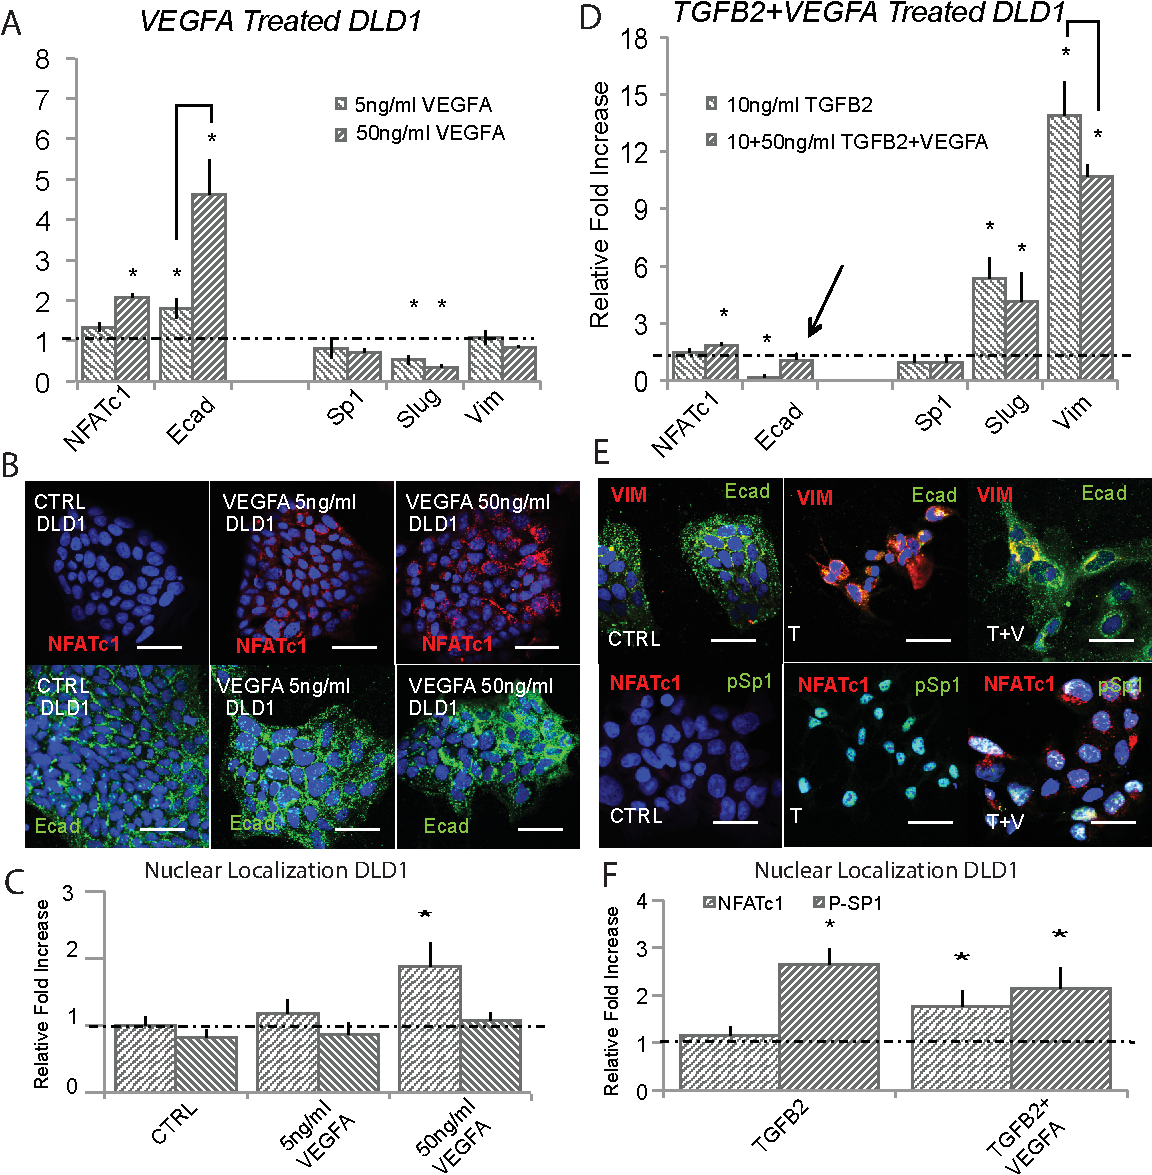
\includegraphics [width=1.0\linewidth] {./figs/Fig-3-Supplemental-DLD1.pdf}
\caption{VEGF-A attenuates TGF-$\beta$1/2 to induce phenotype heterogeneity in DLD1.
(A) In DLD1, we found that 5ng/ml of VEGFA increased NFATc1 and E-cadherin gene expression via qPCR and 50ng/ml potentiated this effect at 48 hrs.
(B - C) These findings were confirmed at the protein level via immunofluorescence, as ecadherin levels and nuclear localization of NFATc1 increased.
(D) Treatment with (10ng/ml) TGF$\beta$2 resulted in mesenchymal transformation as measured via qPCR against target genes Slug, ecadherin, vimentin, Sp1, and NFATc1.
(E - F) Immunofluorescence and nuclear localization revealed a strong presence of phospho-Sp1.
(G) Combination of VEGFA (50ng/ml) and TGF$\beta$2 (10ng/ml) treatment resulted in increased Slug, NFATc1, and vimentin expression, while also increasing ecadherin levels compared to control.
(H) Immunofluorescence confirmed these results, as both ecadherin and vimentin levels were elevated.
(I) A significant increase in nuclear localization of both NFATc1 and phospho-Sp1 were also found.
Magnification, 40x. Scale bars: 50$\mu$m.  C=Control, T=TGF$\beta$2 , V=VEGFA, VI=NFAT inhibitor (VIVIT).
Asterisks signify statistical differences from each other according to a one-way ANOVA with Tukey's post hoc (p$\prec$0.05).}\label{fg:S3}
\end{figure}

\begin{figure}
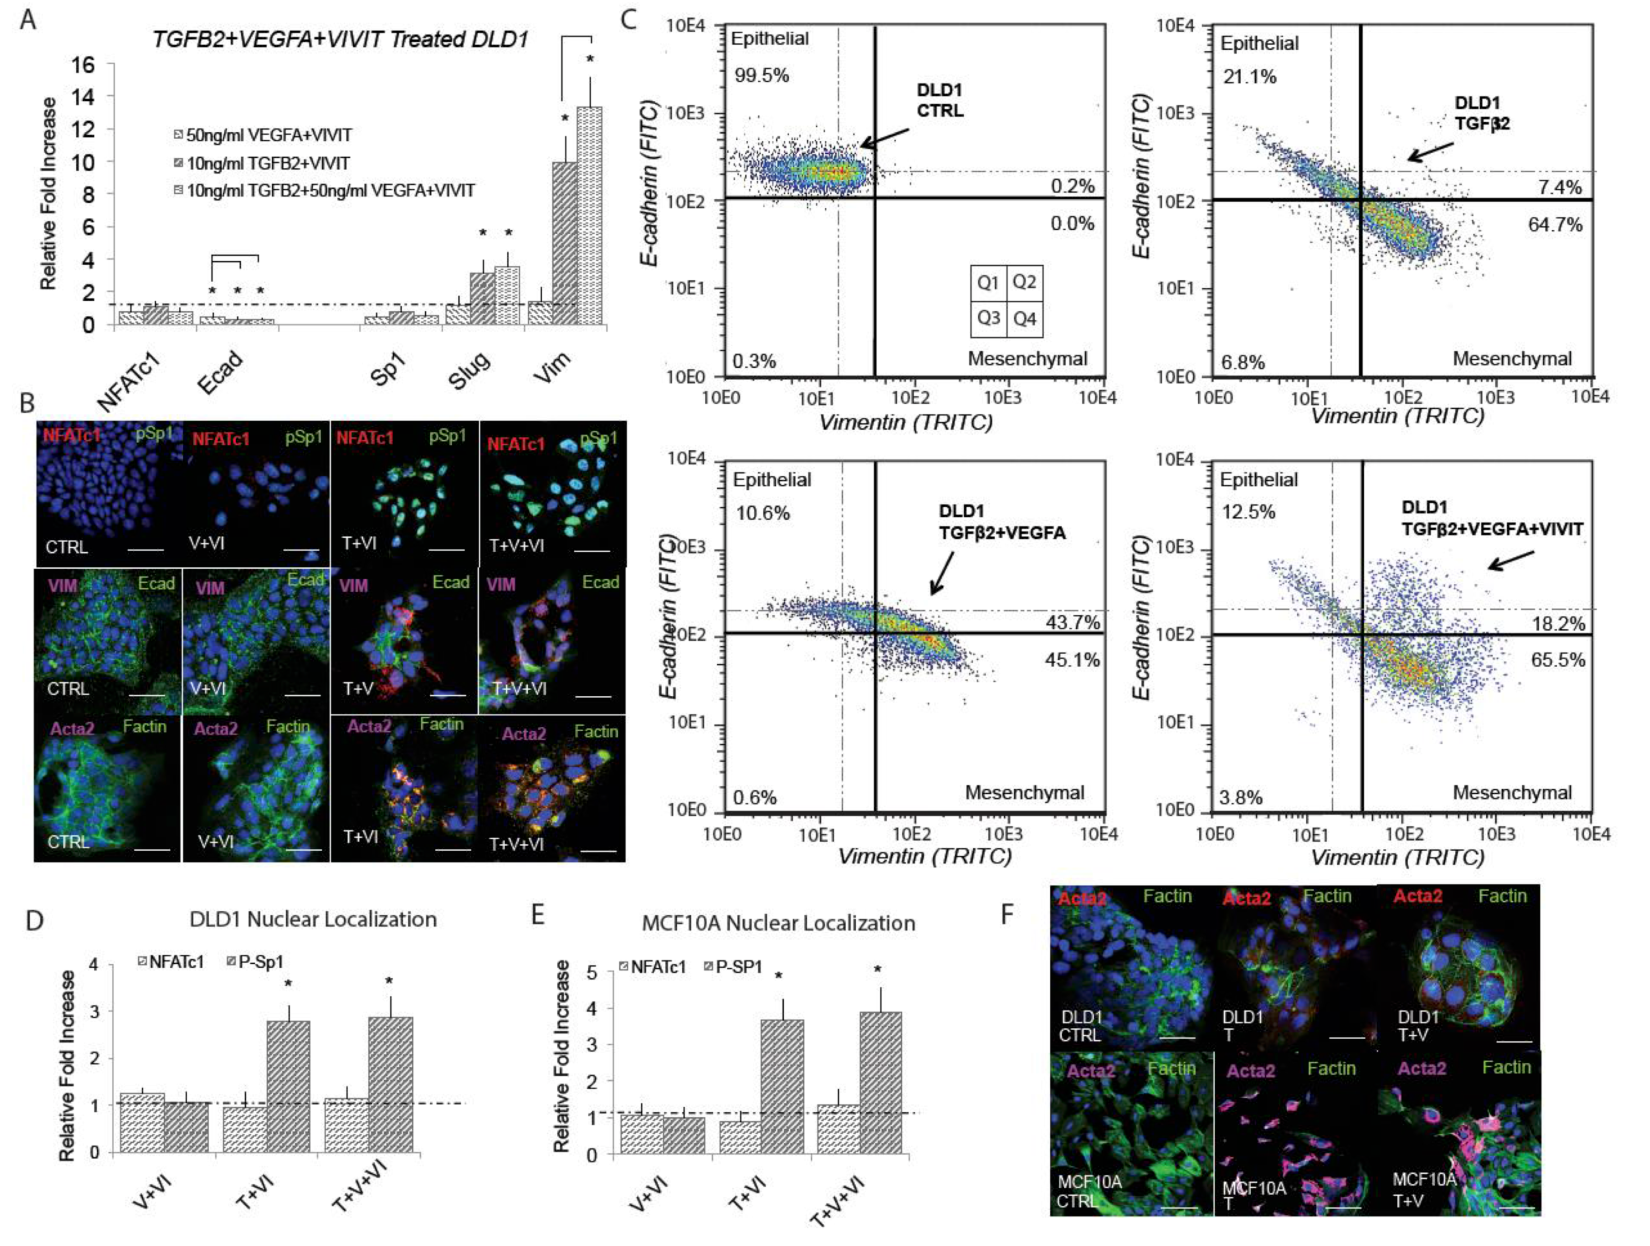
\includegraphics [width=1.0\linewidth] {./figs/Fig-4-Supplemental-DLD1-FlowCyto.pdf}
\caption{E-cadherin expression is dependent upon NFAT activity in DLD1.
(A) Treatment with VEGFA (50ng/ml) and NFAT inhibitory peptide VIVIT (10$\mu$M) resulted in significantly reduced ecadherin expression (qRT-PCR at 48hrs).
Addition of TGF$\beta$2 (10ng/ml) and VIVIT resulted in increased Slug and vimentin expression, while inhibiting ecadherin levels.
Combined TGF$\beta$2, VEGFA, and VIVIT treatment resulted in target genes Slug and vimentin expression increased, while inhibiting ecadherin levels.
No change in Sp1 or NFATc1 expression was found.
(B) These findings were confirmed via immunofluorescence as the VIVIT inhibitors was shown to inhibit ecadherin levels in all three cases.
We also found no change in gene or nuclear localization of NFATc1 in all three cases, while phospho-Sp1 was found to increase in both TGF$\beta$ conditions.
(C) Quantitative flow cytometry also confirmed this trend.
(D,E)  TGF$\beta$2, VEGFA and VIVIT treatment in DLD1 and MCF10A resulted in no change of Sp1 expression or NFATc1 expression.
(F)  Likewise, no change in nuclear localization of NFAT in all three cases, however phospho-Sp1 was found to increase in both TGF$\beta$ conditions.
Magnification, 40x. Scale bars: 50$\mu$m.  C=Control, T=TGF$\beta$2 , V=VEGFA, VI= NFAT inhibitor (VIVIT).
Asterisks signify statistical differences from each other according to a one-way ANOVA with Tukey's post hoc (p$\prec$0.05).}\label{fg:S4}
\end{figure}

\newpage

\begin{figure}
	\center
	\includegraphics [width=0.75\linewidth] {./figs/Fig-Supplemental-Data-VEGFA.pdf}
	\caption{VEGF-A qPCR data used to hand fit VEGF enhancement of E-cadherin expression. mRNA was harvested after 3hr and 48hr timepoint.}\label{fg:VEGFA-Data}
\end{figure}


%\bibliography{References_v1}

% in place ref %

@article{IMAGEJ,
	Author = {Abramoff, M.D. and Magelhaes, P.J. and Ram, S.J.},
	Date-Added = {2011-11-07 13:49:32 -0500},
	Date-Modified = {2011-11-07 13:49:32 -0500},
	Journal = {Biophotonics International,},
	Pages = {36-42},
	Title = {Image Processing with ImageJ},
	Volume = {11},
	Year = {2004}}


